% Standalone figure for freysoldt.tex (Section 2).
% Generated by make_transition_levels.py.
\documentclass[11pt,tikz,border=2pt]{standalone}
\usepackage{amsmath,amssymb}
\usetikzlibrary{arrows.meta, positioning}
\begin{document}
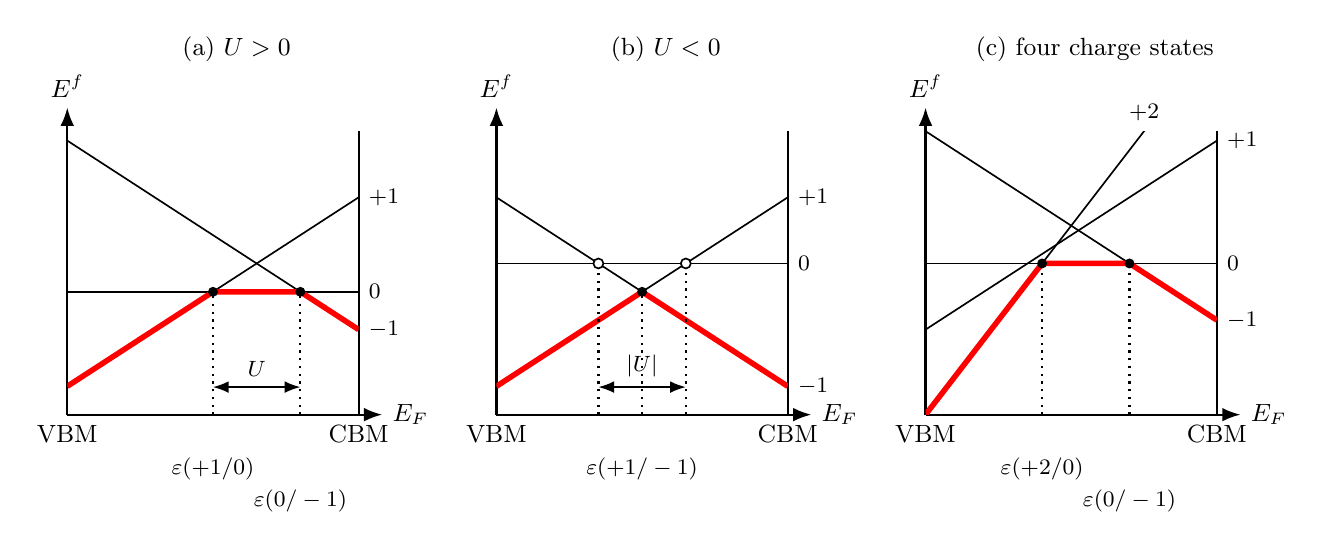
\begin{tikzpicture}[font=\small, >=Latex, line width=0.8pt]
\begin{scope}[xshift=0.0cm]
\draw[->] (0,0) -- (4.00,0) node[right] {$E_F$};
\draw[->] (0,0) -- (0,3.90) node[above] {$E^f$};
\draw (3.700,0) -- (3.700,3.600);
\node[below] at (0,0) {VBM};
\node[below] at (3.700,0) {CBM};
\node[anchor=south] at (2.150,4.35) {(a) $U>0$};
\begin{scope}\clip (0,0) rectangle (3.700,3.600);
\draw[line width=0.6pt] (0.000,0.360) -- (3.700,2.760);
\draw[line width=0.6pt] (0.000,1.560) -- (3.700,1.560);
\draw[line width=0.6pt] (0.000,3.480) -- (3.700,1.080);
\draw[red, line width=2.0pt] (0.000,0.360) -- (1.850,1.560) -- (2.960,1.560) -- (3.700,1.080);
\end{scope}
\node[right, font=\footnotesize] at (3.700,2.760) {$+1$};
\node[right, font=\footnotesize] at (3.700,1.560) {$0$};
\node[right, font=\footnotesize] at (3.700,1.080) {$-1$};
\draw[dotted] (1.850,0) -- (1.850,1.560);
\fill (1.850,1.560) circle (1.8pt);
\node[below, font=\footnotesize] at (1.850,-0.42) {$\varepsilon(+1/0)$};
\draw[dotted] (2.960,0) -- (2.960,1.560);
\fill (2.960,1.560) circle (1.8pt);
\node[below, font=\footnotesize] at (2.960,-0.82) {$\varepsilon(0/-1)$};
\draw[<->, line width=0.6pt] (1.850,0.350) -- (2.960,0.350);
\node[above, font=\footnotesize] at (2.405,0.350) {$U$};
\end{scope}
\begin{scope}[xshift=5.45cm]
\draw[->] (0,0) -- (4.00,0) node[right] {$E_F$};
\draw[->] (0,0) -- (0,3.90) node[above] {$E^f$};
\draw (3.700,0) -- (3.700,3.600);
\node[below] at (0,0) {VBM};
\node[below] at (3.700,0) {CBM};
\node[anchor=south] at (2.150,4.35) {(b) $U<0$};
\begin{scope}\clip (0,0) rectangle (3.700,3.600);
\draw[line width=0.6pt] (0.000,0.360) -- (3.700,2.760);
\draw[line width=0.6pt] (0.000,1.920) -- (3.700,1.920);
\draw[line width=0.6pt] (0.000,2.760) -- (3.700,0.360);
\draw[red, line width=2.0pt] (0.000,0.360) -- (1.850,1.560) -- (3.700,0.360);
\end{scope}
\node[right, font=\footnotesize] at (3.700,2.760) {$+1$};
\node[right, font=\footnotesize] at (3.700,1.920) {$0$};
\node[right, font=\footnotesize] at (3.700,0.360) {$-1$};
\draw[dotted] (1.850,0) -- (1.850,1.560);
\fill (1.850,1.560) circle (1.8pt);
\node[below, font=\footnotesize] at (1.850,-0.42) {$\varepsilon(+1/-1)$};
\draw[<->, line width=0.6pt] (2.405,0.350) -- (1.295,0.350);
\node[above, font=\footnotesize] at (1.850,0.350) {$|U|$};
\draw[dotted] (2.405,0) -- (2.405,1.920);
\draw[line width=0.6pt, fill=white] (2.405,1.920) circle (1.8pt);
\draw[dotted] (1.295,0) -- (1.295,1.920);
\draw[line width=0.6pt, fill=white] (1.295,1.920) circle (1.8pt);
\end{scope}
\begin{scope}[xshift=10.9cm]
\draw[->] (0,0) -- (4.00,0) node[right] {$E_F$};
\draw[->] (0,0) -- (0,3.90) node[above] {$E^f$};
\draw (3.700,0) -- (3.700,3.600);
\node[below] at (0,0) {VBM};
\node[below] at (3.700,0) {CBM};
\node[anchor=south] at (2.150,4.35) {(c) four charge states};
\begin{scope}\clip (0,0) rectangle (3.700,3.600);
\draw[line width=0.6pt] (0.000,0.000) -- (3.700,4.800);
\draw[line width=0.6pt] (0.000,1.080) -- (3.700,3.480);
\draw[line width=0.6pt] (0.000,1.920) -- (3.700,1.920);
\draw[line width=0.6pt] (0.000,3.600) -- (3.700,1.200);
\draw[red, line width=2.0pt] (0.000,0.000) -- (1.480,1.920) -- (2.590,1.920) -- (3.700,1.200);
\end{scope}
\node[above, font=\footnotesize] at (2.775,3.600) {$+2$};
\node[right, font=\footnotesize] at (3.700,3.480) {$+1$};
\node[right, font=\footnotesize] at (3.700,1.920) {$0$};
\node[right, font=\footnotesize] at (3.700,1.200) {$-1$};
\draw[dotted] (1.480,0) -- (1.480,1.920);
\fill (1.480,1.920) circle (1.8pt);
\node[below, font=\footnotesize] at (1.480,-0.42) {$\varepsilon(+2/0)$};
\draw[dotted] (2.590,0) -- (2.590,1.920);
\fill (2.590,1.920) circle (1.8pt);
\node[below, font=\footnotesize] at (2.590,-0.82) {$\varepsilon(0/-1)$};
\end{scope}
\end{tikzpicture}
\end{document}
